\documentclass{article}
\usepackage{amsmath, amssymb, amsfonts, amsthm}
\usepackage{cancel}
\usepackage[output-complex-root=j]{siunitx}
\usepackage[american, nooldvoltagedirection]{circuitikz}
\usepackage{bm}
\usepackage{listings}
\usepackage{graphicx}
\usepackage{fullpage}
\usepackage{hyperref}

\renewcommand{\thesection}{\arabic{section}}
\renewcommand{\thesubsection}{\thesection.\alph{subsection}}
\renewcommand{\thesubsubsection}{\thesubsection.\roman{subsubsection}}

\newtheorem{theorem}{Theorem}

\newcommand{\unit}[1]{\bm{\hat{#1}}}
\newcommand{\iprod}[2]{\left\langle #1, #2 \right\rangle}
\newcommand{\tpose}[1]{\left[#1\right]^{\! \top} \!\!}
\newcommand{\diff}[1]{\frac{d}{d #1}}

\lstset{
    language=Python,
    tabsize=4,
    basicstyle=\ttfamily,
    numbers=left,
    numberstyle=\ttfamily,
    keywordstyle=\color{blue},
    frame=single
}

\title{ASTRO7A PS02}
\author{Bryan Ngo}
\date{2020-09-07}

\begin{document}

\maketitle

\section{Sunlight in Berkeley}

\subsection{}

\begin{center}
    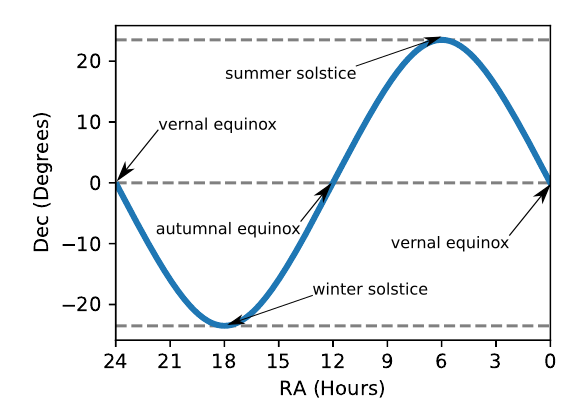
\includegraphics[width=0.8\textwidth]{q1.png}
\end{center}

\subsection{}

\begin{center}
    \begin{tabular}{||c|c|c||}
        \hline
        Position & Right Ascension & Declination \\
        \hline
        Vernal Equinox & \SI{122.27}{\degree} & \SI{-37.87}{\degree} \\
        Winter Solstice & \SI{212.27}{\degree} & \SI{-61.37}{\degree} \\
        Autumnal Equinox & \SI{302.27}{\degree} & \SI{-37.87}{\degree} \\
        Summer Solstice & \SI{32.27}{\degree} & \SI{-14.37}{\degree} \\
        \hline
    \end{tabular}
\end{center}

\subsection{}

If there was a \SI{42}{\degree} orbital tilt, the sun's ecliptic would make a sharper angle with the orbital plane than it currently does.
This means that at the solstices, the Sun will appear higher in the sky.
The equinoxes will not change since the Sun intersects the orbital plane at these points.
The new altitudes are
\begin{center}
    \begin{tabular}{||c|c|c||}
        \hline
        Position & Right Ascension & Declination \\
        \hline
        Vernal Equinox & \SI{122.27}{\degree} & \SI{-37.87}{\degree} \\
        Winter Solstice & \SI{212.27}{\degree} & \SI{-79.87}{\degree} \\
        Autumnal Equinox & \SI{302.27}{\degree} & \SI{-37.87}{\degree} \\
        Summer Solstice & \SI{32.27}{\degree} & \SI{4.13}{\degree} \\
        \hline
    \end{tabular}
\end{center}

\section{A Compact Planetary System}

\subsection{}

The generalized formula of Kepler's third law with units of astronomical units and days is
\begin{equation}
    \left(\frac{P}{365}\right)^2 = a^3 \implies a = \left(\frac{P}{365}\right)^{\frac{3}{2}}
\end{equation}
From there, we can use the equation to determine the periastron and apastron to be, respectively,
\begin{align}
    r_p &= \left.\frac{a (1 - e^2)}{1 + e \cos(\theta)}\right|_{\theta=0} = \frac{a (1 - e^2)}{1 + e} = a (1 - e) \label{eq:periastron} \\
    r_a &= \left.\frac{a (1 - e^2)}{1 + e \cos(\theta)}\right|_{\theta=\SI{\pi}{\radian}} = \frac{a (1 - e^2)}{1 - e} = a (1 + e) \label{eq:apastron}
\end{align}
\begin{center}
    \begin{tabular}{||c|c|c|c||}
        \hline
        Planet & Semimajor Axis [\si{\astronomicalunit}] & Periastron Distance [\si{\astronomicalunit}] & Apastron Distance [\si{\astronomicalunit}] \\
        \hline
        b & \num{4.74e-3} & \num{4.53e-3} & \num{4.95e-3} \\
        c & \num{6.74e-3} & \num{6.56e-3} & \num{6.91e-3} \\
        d & \num{1.55e-2} & \num{1.54e-2} & \num{1.56e-2} \\
        e & \num{2.60e-2} & \num{2.28e-2} & \num{2.91e-2} \\
        f & \num{4.58e-2} & \num{4.52e-2} & \num{4.63e-2} \\
        g & \num{0.18} & \num{0.16} & \num{0.21} \\
        \hline
    \end{tabular}
\end{center}

\subsection{}

The two closest planets are planets b and c, with a closest approach distance of only \SI{1.61e-3}{\astronomicalunit}.

\subsection{}

Converting to SI units, our givens are
\begin{align}
    M_b &= 1.9 \cdot \SI{5.9722e+24}{\kilogram} = \SI{1.13e+25}{\kilogram} \\
    M_c &= 2.9 \cdot \SI{5.9722e+25}{\kilogram} = \SI{1.73e+25}{\kilogram} \\
    r_{bc} &= \frac{\SI{1.61e-3}{\cancel\astronomicalunit}}{1} \cdot \frac{\SI{149597870700}{\meter}}{\SI{1}{\cancel\astronomicalunit}} = \SI{2.41e+8}{\meter}
\end{align}
Then, using Newton's law of universal gravitation,
\begin{equation}
    F_{bc} = \frac{G M_b M_c}{r_{bc}^2} = \frac{G (\SI{1.13e+25}{\kilogram}) (\SI{1.73e+25}{\kilogram})}{(\SI{2.41e+8}{\meter})^2} = \SI{2.26e+23}{\newton}
\end{equation}

\subsection{}

Our givens are
\begin{align}
    M_\star &= 0.961 \cdot \SI{1.98847e+30}{\kilogram} = \SI{1.91e+30}{\kilogram}\\
    r_{b\star} &= \frac{\SI{4.53e-3}{\cancel\astronomicalunit}}{1} \cdot \frac{\SI{149597870700}{\meter}}{\SI{1}{\cancel\astronomicalunit}} = \SI{6.78e+8}{\meter}
\end{align}
The force between planet b and its sun is
\begin{equation}
    F_{b\star} = \frac{G M_B M_\star}{r_{b\star}^2} = \frac{G (\SI{1.13e+25}{\kilogram}) (\SI{1.91e+30}{\kilogram})}{(\SI{6.78e+8}{\meter})^2} = \SI{3.15e+27}{\newton}
\end{equation}
Meaning that the ratio between the closest approach and the solar attraction is
\begin{equation}
    \frac{F_{bc}}{F_{b\star}} = \num{7.18e-5}
\end{equation}

\subsection{}

Here, we want \(r_a\) of planet b to equal \(r_p\) of planet c.
Equating \autoref{eq:periastron} and \autoref{eq:apastron},
\begin{align}
    a_b (1 + e_b) &= a_c (1 - e_c) \\
    \Rightarrow e_b &= \frac{a_c}{a_b} (1 - e_c) - 1 \\
    &= 0.385
\end{align}
So the eccentricity increases by \SI{755}{\percent}.

\section{Eccentric Comets}

\end{document}
